\newpage
\section{Đề thi Đại số}
\begin{tcolorbox}[title=\textbf{Bài toán B.1.}]
    Cho $a$ là một số thực, $A$ là ma trận phụ thuộc vào $a$
    $$A = \begin{pmatrix}[]{cccc}
        1 & a+1 & a+2 & 0 \\
        a+3 & 1 & 0 & a+2 \\
        a+2 & 0 & 1 & a+1 \\
        0 & a+2 & a+3 & 1 
    \end{pmatrix}.$$

    \begin{enumerate}
        \item[(a)] Tìm hạng của ma trận $A$ khi $a = -1$.
        \item[(b)] Tìm tất cả các số thực $a$ sao cho $A$ có định thức dương.
        \item[(c)] Biện luận số chiều của không gian nghiệm của hệ phương trình tuyến tính $AX = 0$ theo $a$ (ở đây $X$ là vector cột ứng với các tọa độ lần lượt là $x,\,y,\,z,\,t$). 
    \end{enumerate}
\end{tcolorbox}

\textbf{Lời giải.}

\begin{enumerate}
    \item[(a)] {
        Khi $a = -1$ thì 
        \begin{align*}
            A 
            & = \begin{pmatrix}[]{cccc}
                1 & 0 & 1 & 0 \\
                2 & 1 & 0 & 1 \\
                1 & 0 & 1 & 0 \\
                0 & 1 & 2 & 1 
            \end{pmatrix} \sim \begin{pmatrix}[]{cccc}
                1 & 0 & 1 & 0 \\
                2 & 1 & 0 & 1 \\
                0 & 1 & 2 & 1 \\
                1 & 0 & 1 & 0 
            \end{pmatrix} \sim \begin{pmatrix}[]{cccc}
                1 & 0 & 1 & 0 \\
                0 & 1 & -2 & 1 \\
                0 & 1 & 2 & 1 \\
                0 & 0 & 0 & 0 
            \end{pmatrix} \sim \begin{pmatrix}[]{cccc}
                1 & 0 & 1 & 0 \\
                0 & 1 & -2 & 1 \\
                0 & 0 & 4 & 0 \\
                0 & 0 & 0 & 0 
            \end{pmatrix}.
        \end{align*}

        Từ đây suy ra $\text{r}(A) = 3$.
    }
    \item[(b)] {
        Theo khai triển Laplace, ta có 

        \begin{align*}
            \det (A) 
            & = \begin{vmatrix}[]{ccc}
                1 & 0 & a+2 \\
                0 & 1 & a+1 \\
                a+2 & a+3 & 1 
            \end{vmatrix} - (a+1)\begin{vmatrix}[]{ccc}
                a+3 & 0 & a+2 \\
                a+2 & 1 & a+1 \\
                0 & a+3 & 1 
            \end{vmatrix} + (a+2)\begin{vmatrix}[]{ccc}
                a+3 & 1 & a+2 \\
                a+2 & 0 & a+1 \\
                0 & a+2 & 1 
            \end{vmatrix} \allowdisplaybreaks \\ 
            & = \left(\begin{vmatrix}[]{cc}
                1 & a+1 \\
                a+3 & 1 
            \end{vmatrix} + (a+2)\begin{vmatrix}[]{cc}
                0 & 1 \\
                a+2 & a+3 
            \end{vmatrix}\right) \\
            & \quad - (a+1)\left(\begin{vmatrix}[]{cc}
                a+3 & 0 \\
                a+2 & 1 
            \end{vmatrix} - (a+3)\begin{vmatrix}[]{cc}
                a+3 & a+2 \\
                a+2 & a+1 
            \end{vmatrix}\right) \allowdisplaybreaks \\
            & \quad + (a+2)\left(\begin{vmatrix}[]{cc}
                a+3 & 1 \\
                a+2 & 0 
            \end{vmatrix} - (a+2)\begin{vmatrix}[]{cc}
                a+3 & a+2 \\
                a+2 & a+1 
            \end{vmatrix}\right) \\   
            & = \Big(1-(a+3)(a+1) - (a+2)^2\Big) - (a+1)(a+3) - (a+2)^2 \\ 
            & \quad + \Big((a+1)(a+3) - (a+2)^2\Big)\begin{vmatrix}[]{cc}
                a+3 & a+2 \\
                a+2 & a+1 
            \end{vmatrix} \\
            & = -4a^2 - 16a - 13 - \begin{vmatrix}[]{cc}
                a+3 & a+2 \\
                a+2 & a+1 
            \end{vmatrix} \\
            & = -4a^2 - 16a - 12 \\
            & = -4(a+1)(a+3).
        \end{align*}

        Như vậy $\det (A) > 0 \iff -4(a+1)(a+3) > 0 \iff -3 < a < -1$.
    }
    \item[(c)] {
        Với $a = -1$, theo câu (a) ta có $\text{r}(A) = 3$ nên số chiều của không gian nghiệm bằng $4 - \text{r}(A) = 1$.

        Với $a = -3$, ta có $$A = \begin{pmatrix}[]{cccc}
            1 & -2 & -1 & 0 \\
            0 & 1 & 0 & -1 \\
            -1 & 0 & 1 & -2 \\
            0 & -1 & 0 & 1 
        \end{pmatrix} \sim \begin{pmatrix}[]{cccc}
            1 & -2 & -1 & 0 \\
            0 & 1 & 0 & -1 \\
            0 & -2 & 0 & -2 \\
            0 & 0 & 0 & 0 
        \end{pmatrix} \sim \begin{pmatrix}[]{cccc}
            1 & -2 & -1 & 0 \\
            0 & 1 & 0 & -1 \\
            0 & 0 & 0 & -4 \\
            0 & 0 & 0 & 0 
        \end{pmatrix},$$ từ đây suy ra $\text{r}(A) = 3$ nên số chiều của không gian nghiệm bằng $4 - \text{r}(A) = 1$.

        Với $a \ne -1,\,-3$ thì $\det (A) \ne 0$ nên hệ phương trình $AX = 0$ có nghiệm duy nhất nên số chiều của không gian nghiệm bằng 0.
    }
\end{enumerate}

\begin{tcolorbox}[title=\textbf{Bài toán B.2.}]
    Cho $A,\,B$ là hai ma trận vuông $$A = \begin{pmatrix}[]{cc}
        0 & 2 \\
        1 & 0 
    \end{pmatrix},\,B = \begin{pmatrix}[]{cc}
        0 & -2 \\
        -1 & 0 
    \end{pmatrix}.$$

    \begin{enumerate}
        \item[(a)] Tìm một ma trận thực $P$ có cấp bằng 2, sao cho $P^{-1}AP$ là ma trận đường chéo.
        \item[(b)] Tìm một ma trận thực $R$ có cấp bằng 2, định thức bằng 1, sao cho $R^{-1}AR = B$.
    \end{enumerate}
\end{tcolorbox}

\textbf{Lời giải.}

\begin{enumerate}
    \item[(a)] {
        Xét ma trận $P = \begin{pmatrix}[]{cc}
            \sqrt{2} & -\sqrt{2} \\
            1 & 1
        \end{pmatrix}$ có $\det (P) = 2\sqrt{2} \ne 0$ nên $P$ khả nghịch.
        
        Khi đó $$P^{-1} = \dfrac{1}{\det (P)} \cdot \text{adj}(P) = \dfrac{1}{2\sqrt{2}}\begin{pmatrix}[]{cc}
            1 & \sqrt{2} \\
            -1 & \sqrt{2} 
        \end{pmatrix},$$ trong đó $\text{adj}(P)$ là ma trận phụ hợp của ma trận $P$. 

        Kiểm tra bằng phép nhân ma trận, ta thấy $$P^{-1}AP = \begin{pmatrix}[]{cc}
            \sqrt{2} & 0 \\
            0 & -\sqrt{2} 
        \end{pmatrix}$$ là ma trận đường chéo.
    }
    \item[(b)] {
        Xét ma trận $Q = \begin{pmatrix}[]{cc}
            1 & -2 \\ 
            1 & -1
        \end{pmatrix}$ có $\det (Q) = 1 \ne 0$ nên $Q$ khả nghịch.
        
        Khi đó $$Q^{-1} = \dfrac{1}{\det (Q)} \cdot \text{adj}(Q) = \begin{pmatrix}[]{cc}
            -1 & 2 \\
            -1 & 1
        \end{pmatrix},$$ trong đó $\text{adj}(Q)$ là ma trận phụ hợp của ma trận $Q$. 

        Kiểm tra bằng phép nhân ma trận, ta thấy $$Q^{-1}AQ = \begin{pmatrix}[]{cc}
            0 & -2 \\
            -1 & 0 
        \end{pmatrix} = B.$$
    } 
\end{enumerate}

\textbf{Nhận xét. }Câu (a) là một bài toán chéo hóa ma trận cơ bản. Câu (b) giải được bằng cách đồng nhất hệ số và giải hệ phương trình. Ma trận $Q$ cần tìm có dạng tổng quát $\begin{pmatrix}[]{cc}
    a & b \\
    c & d 
\end{pmatrix}$, khi đó điều kiện đầu tiên là $\det(Q) = 1$ hay $ad - bc = 1$. Ngoài ra, $Q^{-1} = \dfrac{1}{\det (Q)} \cdot \text{adj}(Q) = \text{adj}(Q) = \begin{pmatrix}[]{cc}
    d & -b \\
    -c & a 
\end{pmatrix}$. Khi đó bằng phép nhân ma trận, ta có $Q^{-1}AQ = \begin{pmatrix}[]{cc}
    2cd-ab & 2d^2-b^2 \\
    a^2-2c^2 & ab-2cd 
\end{pmatrix}$ nên từ đó ta phải có $$\begin{pmatrix}[]{cc}
    2cd-ab & 2d^2-b^2 \\
    a^2-2c^2 & ab-2cd 
\end{pmatrix} = \begin{pmatrix}[]{cc}
    0 & -2 \\
    -1 & 0 
\end{pmatrix}.$$ 

Ta chọn $a,\,b,\,c,\,d$ thỏa mãn hệ phương trình $$\begin{cases}
    ad - bc = 1 \\
    2cd - ab = 0 \\
    2d^2 - b^2 = -2 \\
    a^2 - 2c^2 = -1 \\
    ad - 2cd = 0
\end{cases},$$
từ đó tìm được một bộ $(a,\,b,\,c,\,d)$ thỏa mãn hệ phương trình trên là $(1,\,-2,\,1,\,-1)$.

\begin{tcolorbox}[title=\textbf{Bài toán},breakable]
    Có 200 con muỗi trong một căn hộ gồm 4 phòng với hệ thống cửa nối các phòng như hình vẽ.

    \begin{center}
        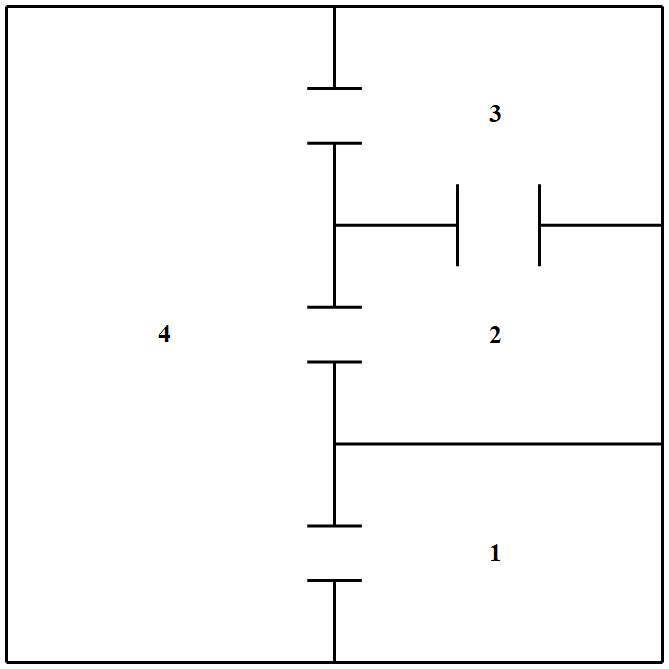
\includegraphics[width=0.5\textwidth]{Figures/01.png}
    \end{center}
    
    Biết rằng, mỗi phút, mỗi con muỗi chỉ ở lại trong phòng nó đang ở hoặc bay sang một phòng bên cạnh. Ngoài ra, người ta thống kê được rằng, với mỗi phòng, có 40\% số muỗi ở lại phòng đó, còn trong số muỗi bay ra khỏi phòng thì số lượng muỗi bay sang mỗi phòng bên cạnh đó là bằng nhau. Chẳng hạn, trong số các con muỗi bay từ phòng 3 sang phòng khác, thì có một nửa bay sang phòng 2, một nửa sang phòng 4.
    
    \begin{enumerate}
        % \begin{multicols}{2}
            \item {Giả sử sau một phút số muỗi ở các phòng 1, phòng 2, phòng 3 và phòng 4 tương ứng là 24, 50, 52 và 74. Tính số muỗi ở mỗi phòng tại thời điểm ban đầu.}
            \item {Gọi trạng thái ổn định là trạng thái mà kể từ đó trở đi số muỗi ở mỗi phòng đều không đổi. Tính số lượng muỗi tương ứng của mỗi phòng tại trạng thái ổn định đó.}         
        % \end{multicols}
    \end{enumerate}
\end{tcolorbox}

\textbf{Lời giải.}

Gọi $a_0,\,b_0,\,c_0,\,d_0$ lần lượt là số muỗi ban đầu của phòng 1, 2, 3, 4; $a_n,\,b_n,\,c_n,\,d_n$ lần lượt là số muỗi của phòng 1, 2, 3, 4 sau phút thứ $n$.

Nhận xét rằng sau mỗi phút, phòng 1 có 40\% số muỗi ở lại, cùng với 20\% số muỗi của phòng 4 bay ra (do 60\% số muỗi phòng 4 bay sang phòng 1, 2, 3) nên ta có phương trình $$a_{n+1} = 0.4a_n + 0.2d_n.$$

Lập luận tương tự, ta thiết lập được hệ phương trình $$\begin{cases}
    a_{n+1} = 0.4a_n + 0.2d_n \\
    b_{n+1} = 0.4b_n + 0.3c_n + 0.2d_n \\
    c_{n+1} = 0.3b_n + 0.4c_n + 0.2d_n \\
    d_{n+1} = 0.6a_n + 0.3b_n + 0.3c_n + 0.4d_n 
\end{cases}.$$

\begin{enumerate}
    \item[(a)] {
        Theo giả thiết, ta có 
        $$\begin{cases}
            0.4a_0 + 0.2d_0 = 24 \\
            0.4b_0 + 0.3c_0 + 0.2d_0 = 50 \\
            0.3b_0 + 0.4c_0 + 0.2d_0 = 52 \\
            0.6a_0 + 0.3b_0 + 0.3c_0 + 0.4d_0 = 74
        \end{cases}.$$

        Xét ma trận bổ sung và thực hiện biến đổi sơ cấp theo dòng 

        \begin{align*}
            \begin{pmatrix}[]{cccc|c}
                0.4 & 0 & 0 & 0.2 & 24 \\
                0 & 0.4 & 0.3 & 0.2 & 50 \\
                0 & 0.3 & 0.4 & 0.2 & 52 \\
                0.6 & 0.3 & 0.3 & 0.4 & 74 
            \end{pmatrix} & \sim \begin{pmatrix}[]{cccc|c}
                0.4 & 0 & 0 & 0.2 & 24 \\
                0 & 0.4 & 0.3 & 0.2 & 50 \\
                0 & 0.3 & 0.4 & 0.2 & 52 \\
                0 & 0.3 & 0.3 & 0.1 & 38 
            \end{pmatrix} \sim \begin{pmatrix}[]{cccc|c}
                0.4 & 0 & 0 & 0.2 & 24 \\
                0 & 0.4 & 0.3 & 0.2 & 50 \\
                0 & 0 & 0.175 & 0.05 & 14.5 \\
                0 & 0 & 0.075 & -0.05 & 0.5 
            \end{pmatrix} \\ & \sim \begin{pmatrix}[]{cccc|c}
                0.4 & 0 & 0 & 0.2 & 24 \\
                0 & 0.4 & 0.3 & 0.2 & 50 \\
                0 & 0 & 0.175 & 0.05 & 14.5 \\
                0 & 0 & 0 & -1/14 & -40/7 
            \end{pmatrix}.
        \end{align*}

        Từ đó ta có được $(a_0,\,b_0,\,c_0,\,d_0) = (20,\,40,\,60,\,80)$.
    }
    \item[(b)] {Ở trạng thái ổn định, ta có $$\begin{cases}
        a_{n} = 0.4a_n + 0.2d_n \\
        b_{n} = 0.4b_n + 0.3c_n + 0.2d_n \\
        c_{n} = 0.3b_n + 0.4c_n + 0.2d_n \\
        d_{n} = 0.6a_n + 0.3b_n + 0.3c_n + 0.4d_n 
    \end{cases} \iff \begin{cases}
        0.6a_n - 0.2d_n = 0 \\
        0.6b_n - 0.3c_n - 0.2d_n = 0 \\
        0.3b_n - 0.6c_n + 0.2d_n = 0 \\
        0.6a_n + 0.3b_n + 0.3c_n - 0.6d_n = 0
    \end{cases}.$$
    
    Xét ma trận hệ số và biến đổi sơ cấp theo dòng
    
    \begin{align*}
        \begin{pmatrix}[]{cccc}
            0.6 & 0 & 0 & -0.2 \\
            0 & 0.6 & -0.3 & -0.2 \\
            0 & 0.3 & -0.6 & 0.2 \\
            0.6 & 0.3 & 0.3 & -0.6 
        \end{pmatrix} & \sim \begin{pmatrix}[]{cccc}
            0.6 & 0 & 0 & -0.2 \\
            0 & 0.6 & -0.3 & -0.2 \\
            0 & 0.3 & -0.6 & 0.2 \\
            0 & 0.3 & 0.3 & -0.4 
        \end{pmatrix} \sim \begin{pmatrix}[]{cccc}
            0.6 & 0 & 0 & -0.2 \\
            0 & 0.6 & -0.3 & -0.2 \\
            0 & 0 & -0.45 & 0.3 \\
            0 & 0 & 0.45 & -0.3 
        \end{pmatrix} \\ & \sim \begin{pmatrix}[]{cccc}
            0.6 & 0 & 0 & -0.2 \\
            0 & 0.6 & -0.3 & -0.2 \\
            0 & 0 & -0.45 & 0.3 \\
            0 & 0 & 0 & 0
        \end{pmatrix} \sim \begin{pmatrix}[]{cccc}
            1 & 0 & 0 & -1/3 \\
            0 & 1 & 0 & -2/3 \\
            0 & 0 & 1 & -2/3 \\
            0 & 0 & 0 & 0
        \end{pmatrix}.
    \end{align*}
    
    Từ đó nghiệm tổng quát của hệ phương trình trên là $(a_n,\,b_n,\,c_n,\,d_n) = \left(\dfrac{1}{3}a,\,\dfrac{2}{3}a,\,\dfrac{2}{3}a,\,a\right)$ với mọi số thực $a$. Mặc khác, vì tổng số muỗi trong các phòng không đổi và bằng $24 + 50 + 52 + 74 = 200$ nên $\dfrac{1}{3}a + \dfrac{2}{3}a + \dfrac{2}{3}a + a = 200$, kéo theo $a = 75$. Như vậy số muỗi ở trạng thái ổn định trong phòng 1, 2, 3, 4 lần lượt là 25, 50, 50, 75.}
\end{enumerate}

\textbf{Nhận xét. }Đây là một bài toán Xích Markov chuyển trạng thái cơ bản, mấu chốt là phân tích được các giả thiết của bài toán và suy ra được hệ phương trình truy hồi ở trên. Bài toán dạng này có thể còn có câu hỏi rằng sau $x$ phút (5 phút, 10 phút,...) số muỗi của mỗi phòng tương ứng là bao nhiêu? Để giải quyết bài toán dạng này, ta viết lại hệ phương trình dưới dạng phương trình ma trận như sau 
$$\begin{pmatrix}[]{c}
    a_{n+1} \\ b_{n+1} \\ c_{n+1} \\ d_{n+1}
\end{pmatrix} = \begin{pmatrix}[]{cccc}
    0.4 & 0 & 0 & 0.2 \\
    0 & 0.4 & 0.3 & 0.2 \\
    0 & 0 & 0.175 & 0.05 \\
    0 & 0 & 0 & -1/14 
\end{pmatrix}\begin{pmatrix}[]{c}
    a_{n} \\ b_{n} \\ c_{n} \\ d_{n}
\end{pmatrix} = A\begin{pmatrix}[]{c}
    a_{n} \\ b_{n} \\ c_{n} \\ d_{n}
\end{pmatrix}.$$

Tính số muỗi của từng phòng sau $x$ phút, tức cần tính $$\begin{pmatrix}[]{c}
    a_{x} \\ b_{x} \\ c_{x} \\ d_{x}
\end{pmatrix} = A\begin{pmatrix}[]{c}
    a_{x-1} \\ b_{x-1} \\ c_{x-1} \\ d_{x-1}
\end{pmatrix} = A^2\begin{pmatrix}[]{c}
    a_{x-2} \\ b_{x-2} \\ c_{x-2} \\ d_{x-2}
\end{pmatrix} = \cdots = A^x\begin{pmatrix}[]{c}
    a_{0} \\ b_{0} \\ c_{0} \\ d_{0}
\end{pmatrix},$$ đến đây quy về việc tính lũy thừa ma trận $A^x$ là xong.